\begin{figure}[ht]
	\centering 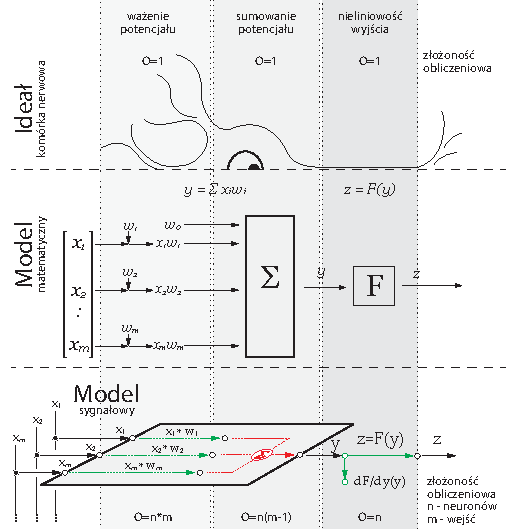
\includegraphics[width=0.9\linewidth]{rysunki/stan_wiedzy_1.jpg} 
	\caption{ Neuron, model matematyczny i sygnałowy  }
	\label{rys:neuronmodel1}
\end{figure}
%ideał - równoległego przetwarzania
%dwukrotne zwiększenie liczby wejść nie powoduje zwiększenia czasu przetwarzania. 
%krok pierwszy: realizacja niezależnego równoległego "ważenia" x1w = x1*w1, x2w = x2*w2, x3w=w3*w3 ... mnożenie o złożoności obliczeniowej: O=1;
%krok drugi: realizacja równoległego wielokanałowego dodawania. sum = x1w + x2w + x3w ..; dodawanie o złożoności obliczeniowej O=1;
%krok trzeci: aktywacja nieliniowa aktywacja F;
Neuron biologiczny przetwarza impulsy wejściowe w trzech krokach:
\begin{itemize}
    \item 
    ważenie wejściowych sygnałów - jest to skomplikowany proces, zmienny w czasie i zależny od historii wcześniejszych impulsów; w modelu matematycznym odpowiada mu mnożenie sygnału wejściowego \(x_i\) przez wielkość wagi \(w_i\) przypisanej do tego sygnału. \( x_iw = x_i * w_i  \)
    
    \item 
    jednoczesne sumowanie potencjałów sygnałów wejściowych - w modelu matematycznym odpowiada mu algebraiczna suma ważonych sygnałów: \( y = \sum x_iw \)

    \item 
    nieliniowa aktywacja - w modelu matematycznym obliczenie wartości funkcji aktywacji \( z = F(y) \)

    \item w modelu sygnałowym dla zwiększenia wydajności zapamiętano wartość pochodnej \(  \frac{\partial F}{\partial y}(z) \) -~zostanie ona wykorzystana w późniejszych obliczeniach w procesie uczenia.
    
\end{itemize} 
 
%W tym rozdziale autor opisze stan wiedzy - matematyczny i sygnałowy model warstwy splotowej CNN oraz warstwy MLP głównych elementów składowych sieci głębokich. A także działanie warstw pomocniczych - łączących, i redukujących. 
%Opisany będzie sposób obliczania odpowiedzi sieci na zaprezentowany wzór - tj. przepływ sygnału wprost. 
%Ponadto opisany zostanie algorytm uczenia "wsteczna propagacją błędu" jako operacja matematyczna i proces przesyłania sygnału wstecz przez sieć.

%*******************
 




\begin{center}
\begin{tabular}{|c|c|c|} 
 \hline
 rodzaj warstwy & funkcja aktywacji  \(  z = F(y) \)  & wartość pochodnej \(  \frac{\partial F}{\partial y} \) \\ 
 logistyczna (sigmoid) &  \( \frac{1}{1+e^-y} \) & \( (z)(1-z) \) \\ 
 ReLU & jeśli y<0 to z=y, jeśli y>=0 to z=0  & jeśli y<0 to 1, jeśli y>=0 to 0 \\ 
  softmax &   \(z_i = \frac{e^{x_i}}{\sum{e^{x_i}}}   \) & dla prawidłowej klasy k:  \(y_k(1-y_k)\),     \\
 softmax &  &  dla pozostałych klas:  \(  -y_i*y_k  \) \\

 \hline 
\end{tabular}
\end{center}


\section{Perceptron warstwowy}
Wejście neuronu przyjmuje wartości  \([ x_1, x_2,  ... , x_m ]\) (wektor), natomiast na wyjściu jednego neuronu pojawia się tylko jeden sygnał wyjściowy \(z\). 
\begin{figure}[ht]
	\centering 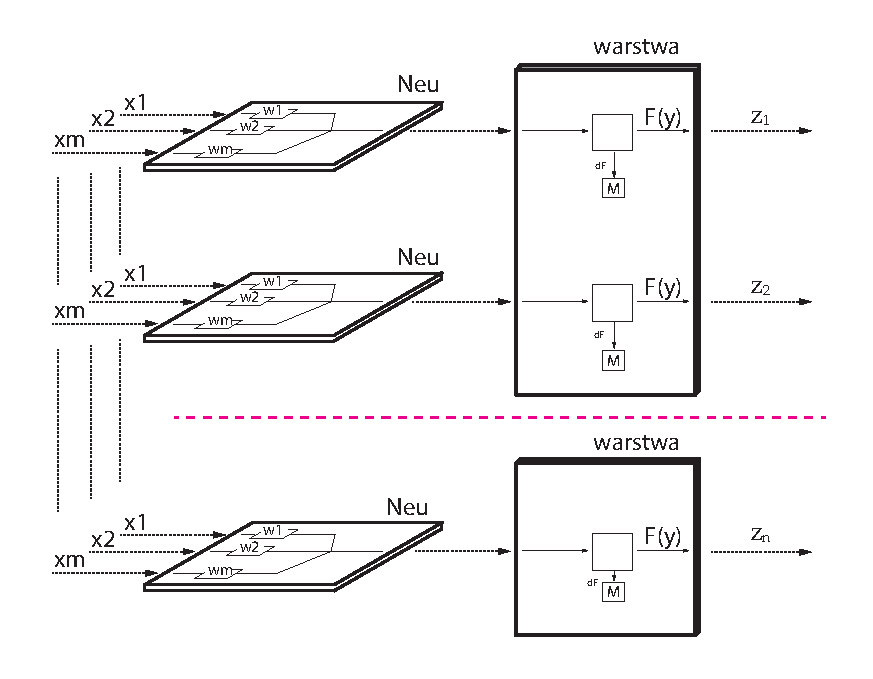
\includegraphics[width=0.75\textwidth]{rysunki/3d.jpg} 
\caption{Przepływ sygnałów przez warstwę w czasie propagacji sygnału "w przód" }
	\label{rys:modelobiektowegoneuronuszkic3}
\end{figure}
 

\begin{figure}[ht]
	\centering \includegraphics[width=0.60\textwidth]{rysunki/forward_layers.jpg} 
	\caption{Propagacja sygnału przez zespół warstw w przód i wstecz}
	\label{rys:operacjesynch2a}
\end{figure}

\section{Proces uczenia MLP}
\begin{figure}[ht]
	\centering 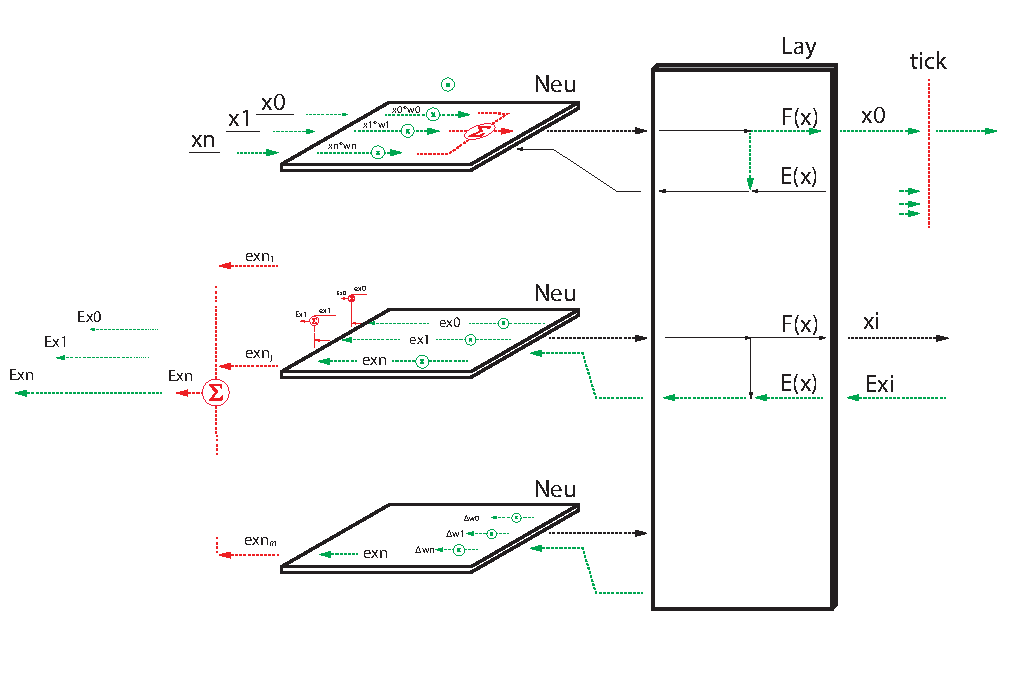
\includegraphics[width=0.93\textwidth]{rysunki/3drev.jpg} 
	\caption{Propagacja wstecz - uczenie sieci. (Operacje niezależne (mnożenie) oznaczone kolorem zielonym i operacje wymagające synchronizacji (dodawanie) oznaczone kolorem czerwonym)}
	\label{rys:operacjesynch2}
\end{figure}
Odpowiedzią sieci jest sygnał wyjściowy ostatniej warstwy. W procesie uczenia z nauczycielem podlega on ocenie, a wielkość błędu sieci jest przekazywana do warstwy wyjściowej. Stosowane są różne strategie wyznaczania wielkości tego wektora. \\
Dla warstwy wyjściowej logistycznej może to być różnica między oczekiwaną odpowiedzią, a odpowiedzią uzyskaną:
\( \left[
                        \begin{matrix}
                             e_{1}\\
                             e_{2}\\
                             e_{m}\\
                        \end{matrix}
                    \right]
                    = 
                     \left[
                        \begin{matrix}
                             s_{1}\\
                             s_{2}\\
                             s_{m}\\
                        \end{matrix}
                    \right]
                    -
                    \left[
                        \begin{matrix}
                             z_{1}\\
                             z_{2}\\
                             z_{m}\\
                        \end{matrix}
                    \right]
\)  gdzie \(S\) jest wektorem oczekiwanym.  
Dla każdej wartości wyjściowej \(z_i\) zostaje zwrócona wielkość błędu \(e_i\), ponadto dla każdej wartości~\(z_i\) zostaje zapamiętana wartość pochodnej \(  \frac{\partial F}{\partial y} \). W procesie uczenia do każdego z neurosumatorów zostaje przekazana odpowiadająca mu wielkość błędu: \( dFe = e_i *  \frac{\partial F}{\partial y} \).  \\
\begin{figure}[ht]
	\centering 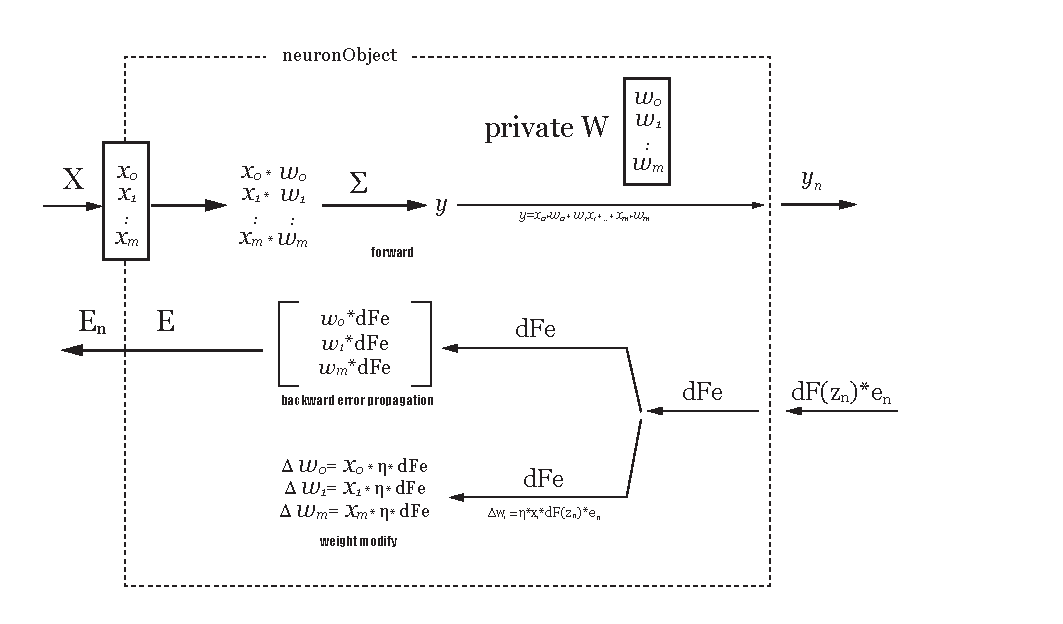
\includegraphics[width=\textwidth]{rysunki/rys1_5.jpg} 
	\caption{Przepływu sygnałów w obiekcie Neurosumator }
	\label{rys:modelobiektowegoneuronuszkic2}
\end{figure}
